\documentclass[a4paper, 12pt]{article}
\usepackage[english]{babel}
\usepackage[a4paper,left=2.5cm, right=2.0cm, top=2.5cm, bottom=2.5cm]{geometry}
\usepackage[utf8]{inputenc}
\usepackage{setspace}
\usepackage{url}
\usepackage{longtable}
\usepackage{lscape}
\usepackage[final]{pdfpages}
\usepackage{graphicx}
\usepackage{colortbl}
\usepackage{multirow}
\usepackage{listings}
\begin{document}
%This file will subsume all of the individual chapters of the project report


%\setstretch{1.50}
\pagestyle{empty}

\begin{center} Project Report \end{center}
\hspace{1cm}
\begin{center} Softwareproject: \end{center}
\begin{center}Spoken Dialog Systems for Elevator Control \end{center}
\begin{center} Universität des Saarlandes \end{center}
\begin{center} Department 4.7 Computational Linguistics and Phonetics \end{center}
\begin{center} Computerlinguistik, B.Sc./M.Sc. \end{center}
\begin{center} Summer term 2015 \end{center} 

\hspace{1cm}
\begin{center}Instructors: Ingmar Steiner, Asad Sayeed, Arif Khan \end{center}

\begin{center} Participants: Anne-Julia Hoffmann, Boyuan Deng, Laura Faust \end{center}


\pagestyle{plain}
\setcounter{page}{1}

%please put in the files you wrote in the corresponding order and space by 
%using \input{filename} so that we can compile the entire project report as one

\section{Dialogue System}

\subsection{ASR}

\subsubsection{Acoustic model}
Training etc.
\subsection{Reverberation recordings in the elevator}

\begin{figure}[h]
\hspace*{3cm}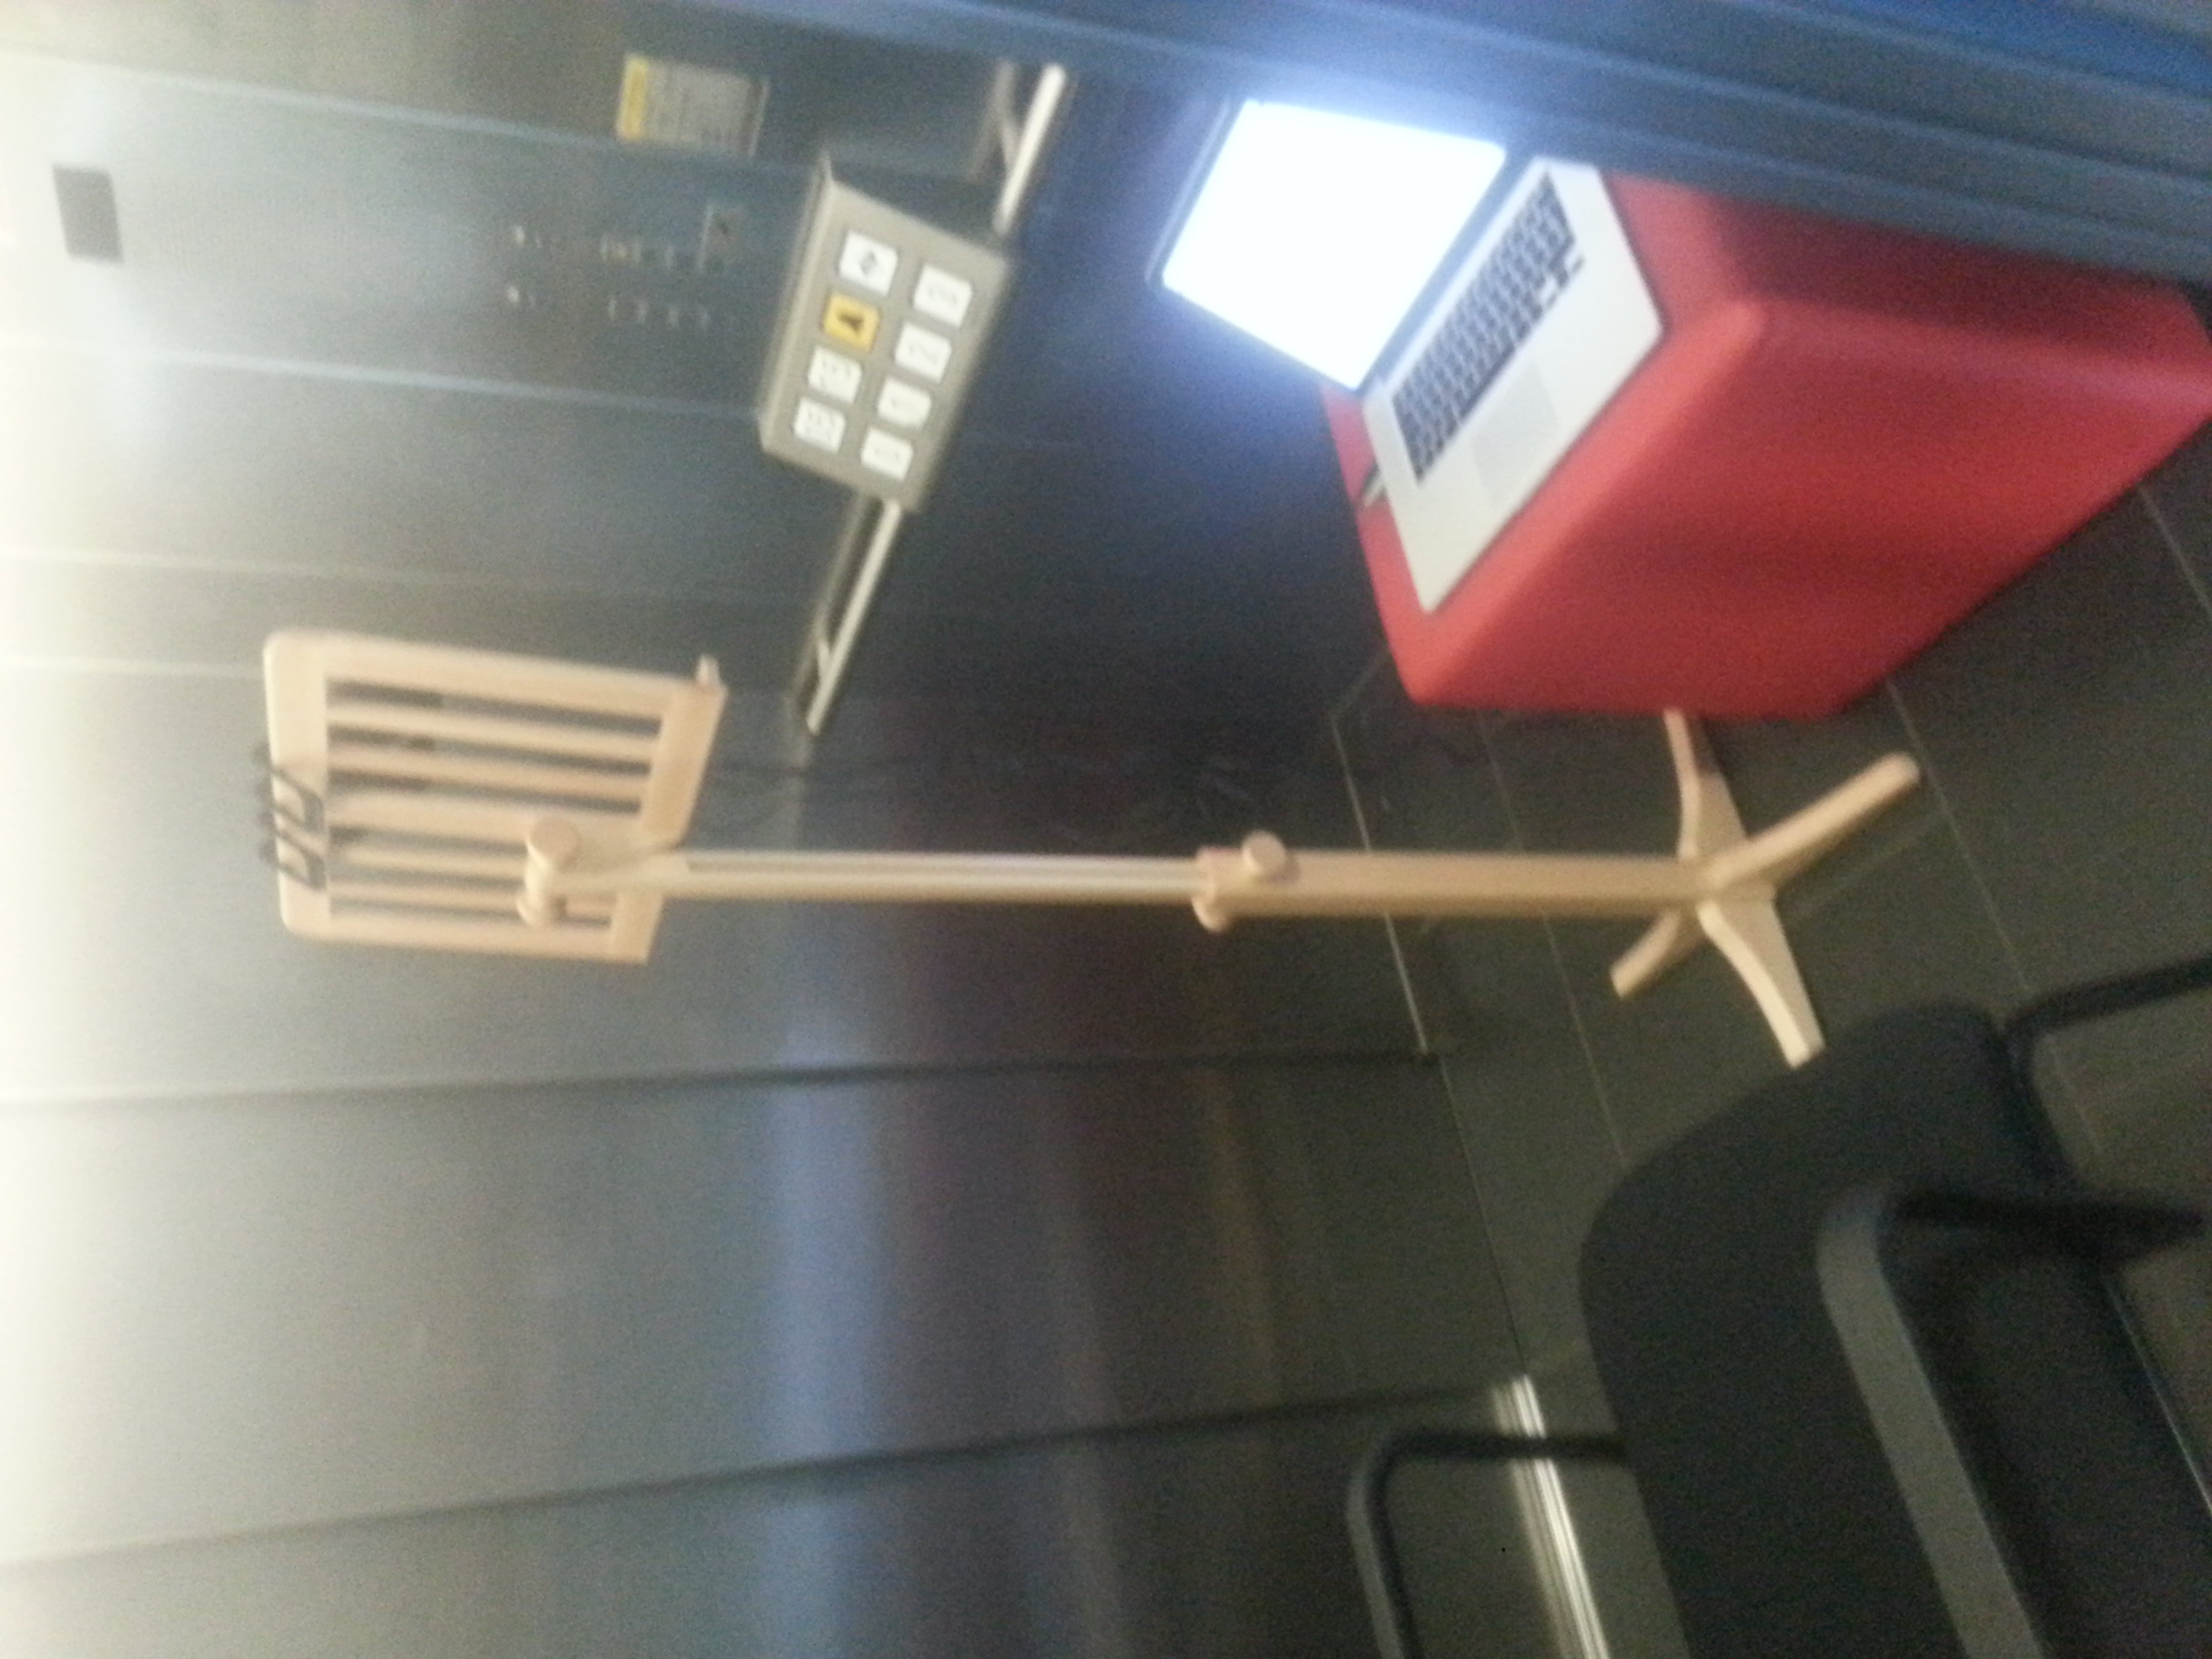
\includegraphics[scale=0.15]{setup_reverberation_rec.jpg}
\caption{Recordings setup.}
\label{fig:recordingsetup}
\end{figure}



\noindent To account for the noise of the elevator, its sound when moving, the sound of the doors opening and closing and the reverberation with open doors on the different floors and other noises from outside of the elevator, recordings were done via the elevator's built-in microphone. 
The setup used for this can be seen in picture \ref{fig:recordingsetup}.
It consisted of two loudspeakers positioned on a music stand at the height of approximately 150cm, at a distance of approximately 20cm from the elevator's microphone. 
The recordings made in the lab were played through the loudspeakers and recorded with Praat via the elevator's microphone. 
While the recordings were being played, the elevator was moved between the floors, its doors were opened and closed and kept with its doors opened and closed on different floors.


\subsubsection{Language model}

%\input{jsgf_summary.tex}

\subsection{Dialog-manager}

The dialog manager is responsible for keeping track of the conversation and deciding the next move of the system for each input. The domain of our project is fairly limited. Most conversational situations consist of the user naming a location and the machine taking the action of moving to that location and reassuring the user that it had understood the command. This can described by deterministic If...then... statements. A dialog manager that models the conversation flow as an deterministic FSA is well-suited for our needs.
When choosing the dialog manager for our project we considered the following factors: It had to be open source, preferably Java, well documented.
We were also looking for code that was actively maintained.
We reviewed a few potential contenders:
\begin{itemize}
\item[IrisTK] \hfill \\
TODO
\item[InproTK] \hfill \\
The most exciting asset of this dialog manager was incremental processing.
The code is well maintained and actively developed. 
However, we failed to build a demo that uses incremental features due to the lack of documentation so we dropped this option.
\item[OpenDial] \hfill \\
OpenDial is probably the most popular open source dialog manager.
After successfully implementing a short domain-relevant demo we opted for this manager.
For more detailed description of OpenDial see next section.

\end{itemize}
\subsubsection{Opendial}
\subsubsection{some Other}

\subsection{TTS}

\section{Implementation details}
\subsection{Raspberry pi}
pi4j, rasberry pi virtualization
\subsection{Serial control of elevator}
\subsection{Testing}
\subsection{Development tools}

\subsubsection{Gradle}
Gradle\footnote{http://gradle.org/} is a build automation tool and simplifies the build process drastically.
Instead of having a readme file that explains how to build the project, building the project is as easy as executing \texttt{./gradlew build} on the command line.

Gradle is configured in the file \texttt{build.gradle}.
Although it looks like a configuration file, it is actually fully functional code written in Groovy\footnote{http://www.groovy-lang.org/}, a programming language based on Java.

We included a Gradle wrapper in the repository.
This file called \texttt{gradlew} (and \texttt{gradle.bat} for windows) download and run the right Gradle version when executed.
It is recommended to use this file instead of using this file instead of any other locally installed Gradle, because it might be another version of Gradle.

The file \texttt{settings.gradle} specifies the gradle project structure by declaring several subprojects.
There is the opendial subproject, which is a copy of the dialog manager OpenDial\footnote{http://www.opendial-toolkit.net/}.
Next we have the pi4j subproject, which is a copy of Pi4j\footnote{http://pi4j.com/}.
We use it for serial port communication.
Next we have the sphinx4 subproject, consisting of sphinx4-core and sphinx4-data, which is a copy of the speech recognition software Sphinx4\footnote{https://github.com/cmusphinx/sphinx4}.
These subprojects are all forked on github from the originals, eventually adapted for our purposes and then included as a Git submodule.
Finally we have a subproject called prompts, that is our own making.
It contains example audio prompts for our application, that are used for the acoustic model training and for testing.

\subsubsection{github}
GitHub is a web platform for collaboration using git, which is a version control system. 
We used this system to allow several people work on the same project at the same time without overwriting each others changes.

For some of our dependencies (Sphinx, pi4j, OpenDial) we used git submodules to include them into our project. 
This gave us the possibility to adapt the original code for our purposes if necessary.
In order to download these dependencies when you clone the repository, you must therefore execute
\begin{lstlisting}[language=bash]
git clone https://github.com/EllaVator/EllaVator.git --recursive
\end{lstlisting}
or init and update all of the subprojects individually.

\subsubsection{Travis}
\subsection{Continuous integration with Travis CI}

Continuous integration is based on the idea that all developers send their changes to a common code repository as soon as possible, as we did on GitHub. 
Additionally these changes should be tested before they are merged into the main code repository. 
In order to do this automatically, it is necessary to automate the build process completely, as we did using Gradle.
If the build succeeds, all unit and integration tests can be executed, which prevents non-working code to enter the main repository if the error is covered by a test case.
This procedure is much better than having each developer running the tests before committing the changes to the main repository for a couple of reasons.
Firstly it does not rely on the developer to run all the tests which can be easily forgotten or skipped because the developer does not see the whole effect his modification has.
Secondly the project is built in a “neutral” environment that should be a close copy of the production environment if possible. 
This way for example code that runs fine on the developer's Windows machine but not on Linux can be detected.

As it integrates seamlessly into GitHub, we decided to use Travis CI as our continuous integration service. Each pull request gets marked by colors: yellow means the build is still running, red means failed build or failed test, green says everything is OK. In each pull request there is a link to Travis that gives details about the build process, too.

Travis is configured by a file named \texttt{.travis.yml} in the root directory of the project. 
It is not even necessary to specify that the build process is handled by Gradle.
Travis can detect this automatically, given that we specify groovy as our project language (\texttt{language: groovy}).
We needed to use Java 8 because this is a minimum requirement for Opendial.
Also, Travis must install the \texttt{sox} command, which is used to extract single sentences from our test audio files in the prompts subproject.
Finally, we cache the gradle files to speed up the build process (otherwise the Gradle wrapper will download Gradle every time).

Each developer can add Travis to his own repositories, too.
That way failures can be detected even before sending a pull request.
Travis can be activated by signing up on \url{https://travis-ci.org/} using your GitHub account.
Then go to your profile page on Travis and activate the GitHub repositories you want to be watched (which must contain a \texttt{.travis.yml} file).
From then on every push to these repositories will trigger Travis to build and run tests and send an email about the result.



\include{bibliography}

\end{document}
